\documentclass[hyperref={pdfpagemode=FullScreen}]{beamer}
\usepackage[utf8]{inputenc}
\usepackage{multicol}
\usepackage{graphicx}
\usepackage{ragged2e}
\title{Azerbaijan}
\usetheme{Madrid}
\usecolortheme{beaver}
\title{AZERBAIJAN}
\author{Rashad Mahmudov}
\date{3 May 2020}

\begin{document}

\begin{frame}
\titlepage
\end{frame}

\setlength{\columnsep}{0.7cm}
\begin{frame}{Location}

\begin{multicols}{2}

\justifying 
Republic of Azerbaijan, is a country in the South Caucasus.


It is bounded by the Caspian Sea to the east, Russia to the north, Georgia to the west and Iran to the south. 

\columnbreak
\hspace{.2cm}
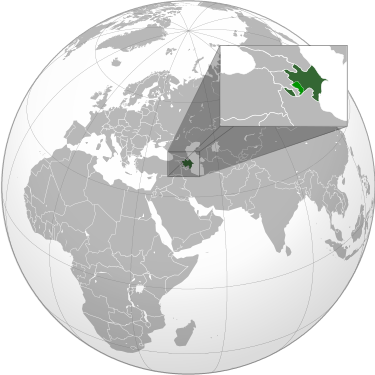
\includegraphics[scale=.32]{img/aze01.png}
\end{multicols}
\end{frame}


\begin{frame}{History}
\begin{alertblock}{Antiquity}
\justifying The earliest evidence of human in  Azerbaijan dates back to the late Stone Age and is related to the Guruchay culture.
\end{alertblock}
\end{frame}


\begin{frame}{History}
    \begin{figure}
        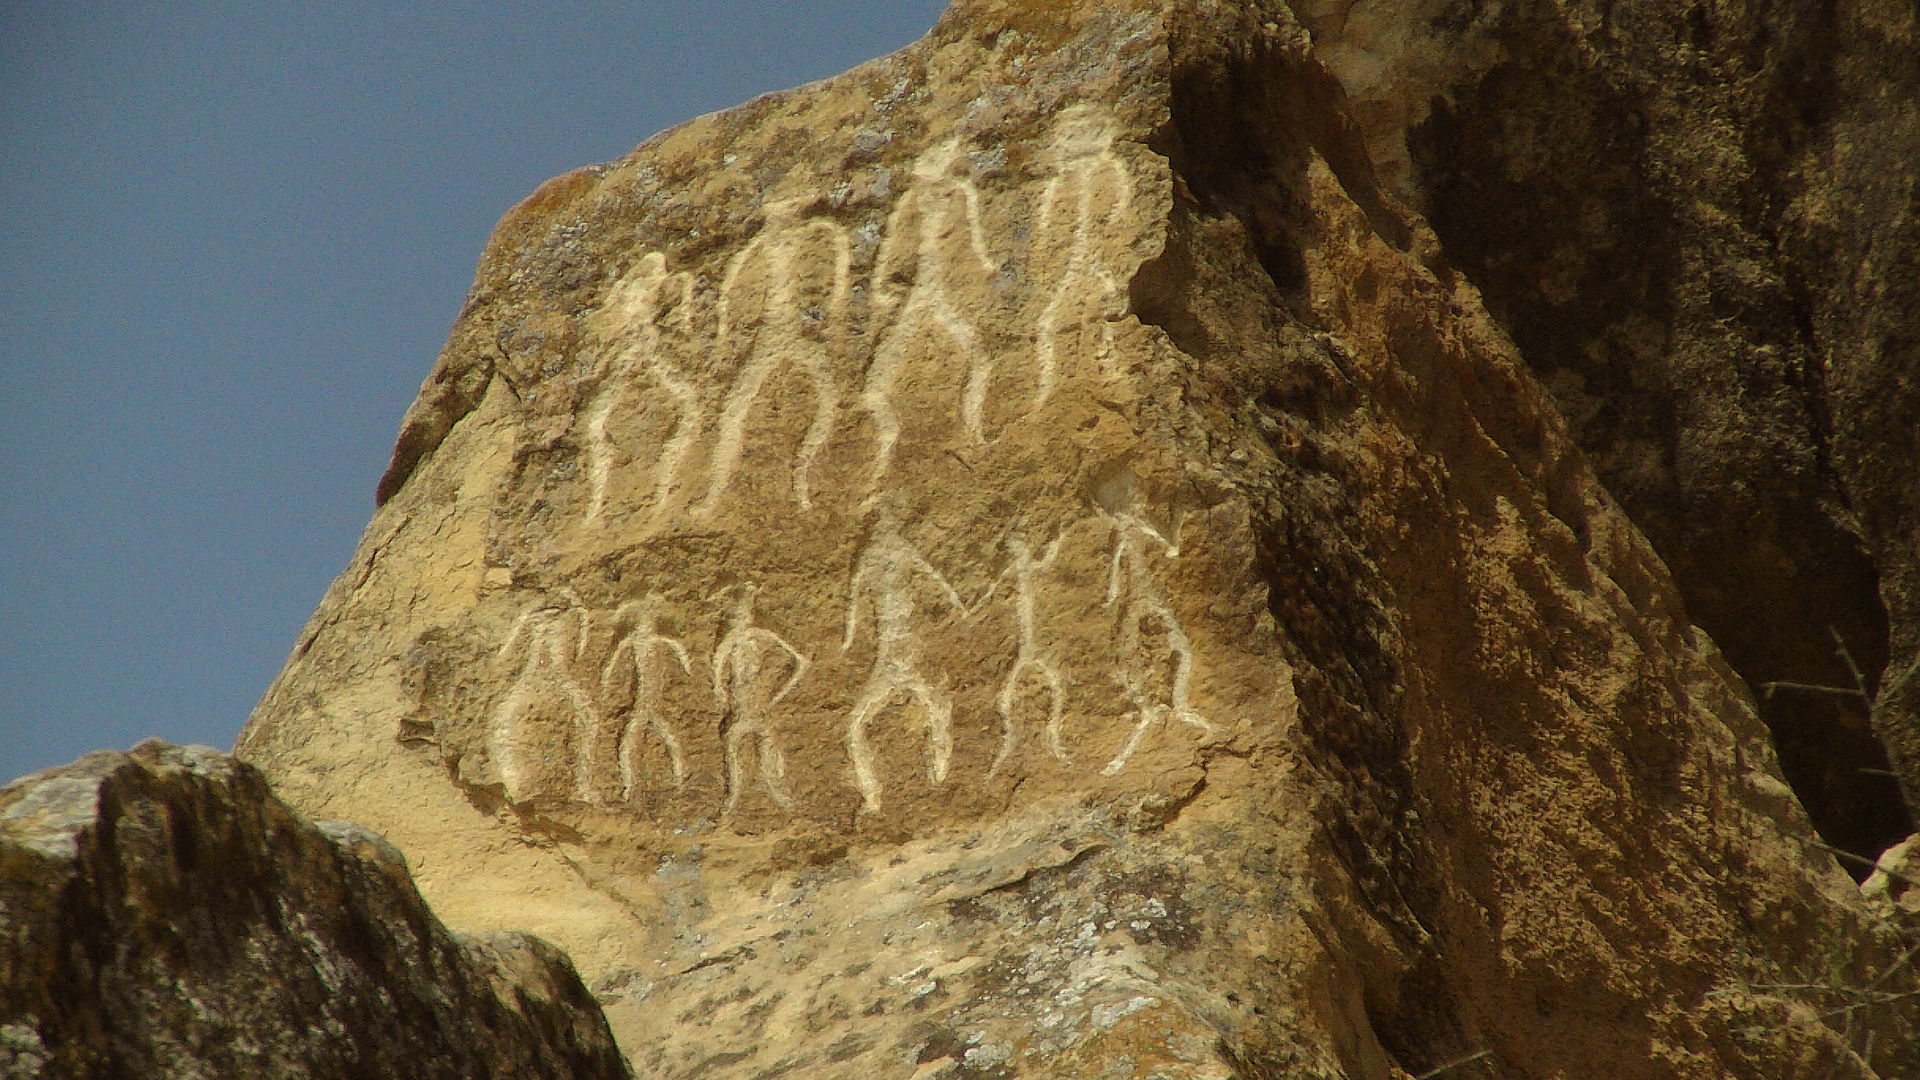
\includegraphics[width=11cm, height=6cm]{img/aze02.jpg}
        \caption{Azokh Cave} 
    \end{figure}
\end{frame}

\begin{frame}{Cities}
\begin{alertblock}{Baku}
\justifying Baku, the capital city of Azerbaijan. It is the biggest city in Azerbaijan and the largest city in the Caucasus region. Baku population - 2,262,600
\end{alertblock}
\end{frame}

\begin{frame}{
\includegraphics[width=.9cm, height=1.2cm]{img/baku04.png}}
    \begin{figure}
        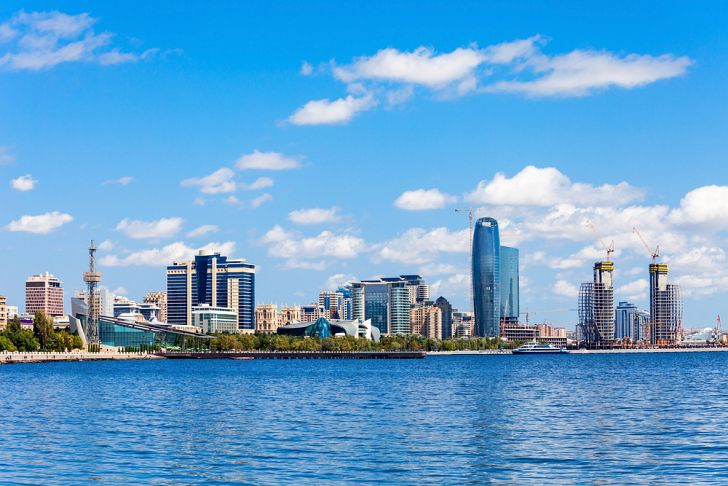
\includegraphics[width=11cm, height=6cm]{img/baku01.jpg}
        \caption{Baku See View} 
    \end{figure}
\end{frame}

\begin{frame}{
\includegraphics[width=.9cm, height=1.2cm]{img/baku04.png}}
    \begin{figure}
        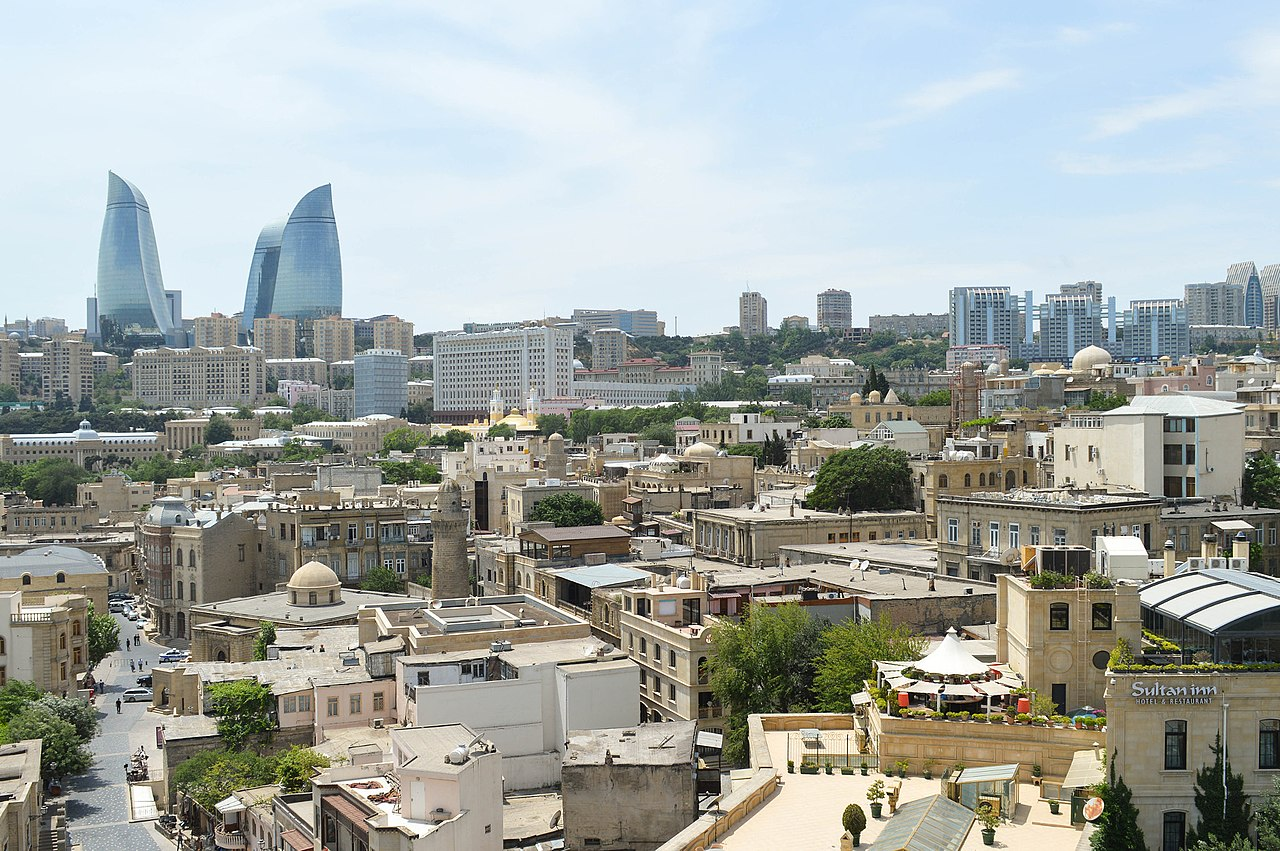
\includegraphics[width=11cm, height=6cm]{img/baku02.jpeg}
        \caption{Baku Old City} 
    \end{figure}
\end{frame}

\begin{frame}{
\includegraphics[width=.9cm, height=1.2cm]{img/baku04.png}}
    \begin{figure}
        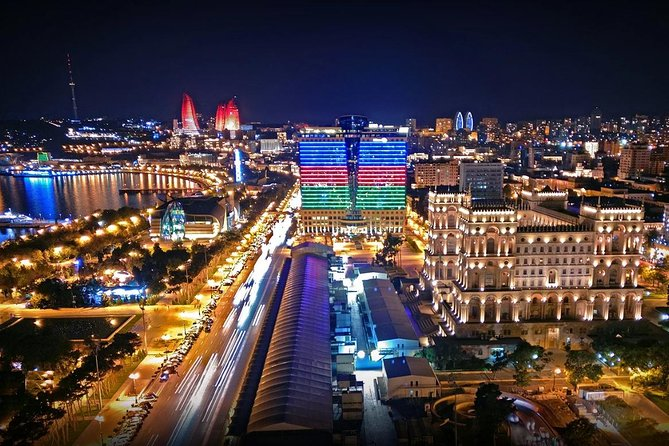
\includegraphics[width=11cm, height=6cm]{img/baku03.jpg}
        \caption{Baku Night View} 
    \end{figure}
\end{frame}

\begin{frame}{Cities}
\begin{alertblock}{Ganja}
\justifying Ganja is the second largest city of Azerbaijan.
Ganja is one of the oldest cities in the Caucasus. Ganja population - 332,600.
\end{alertblock}
\end{frame}

\begin{frame}{
\includegraphics[width=.9cm, height=1.2cm]{img/gence04.png}}
    \begin{figure}
        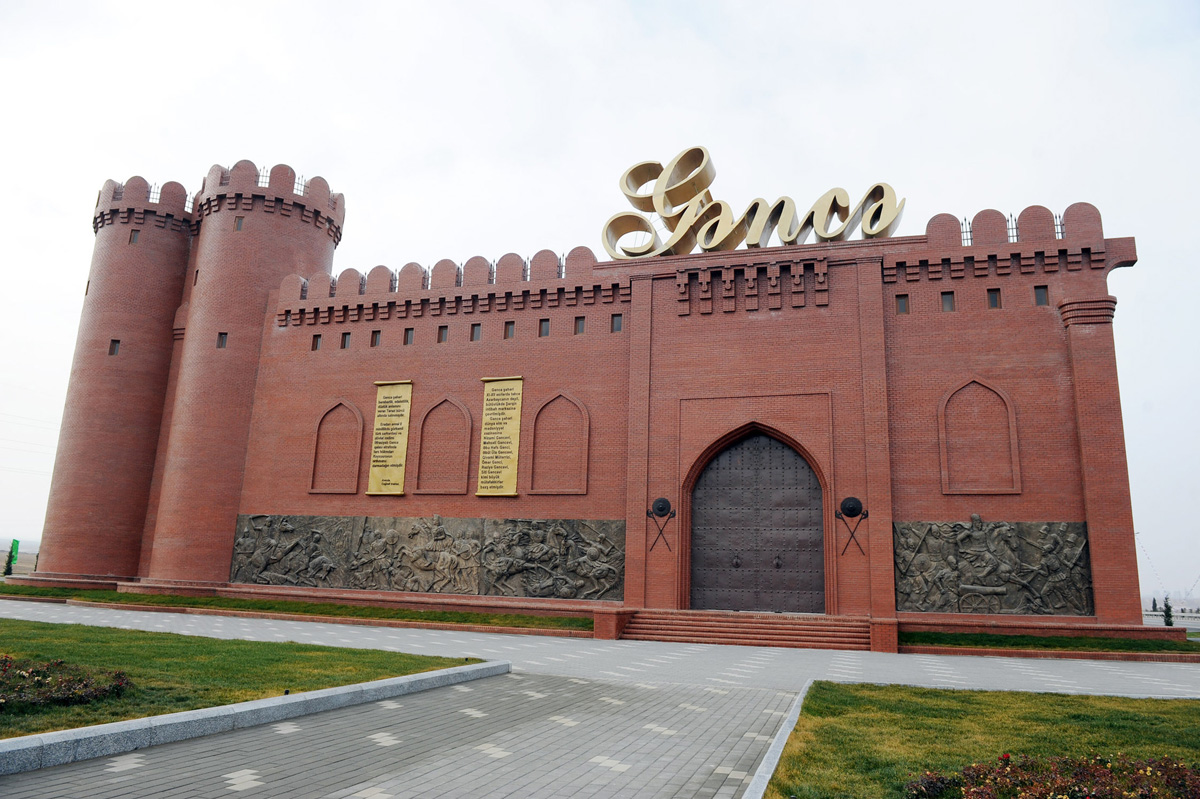
\includegraphics[width=11cm, height=6cm]{img/gence01.jpg}
        \caption{Ganja Fortress Gates} 
    \end{figure}
\end{frame}

\begin{frame}{
  
\includegraphics[width=.9cm, height=1.2cm]{img/gence04.png}
}
    \begin{figure}
        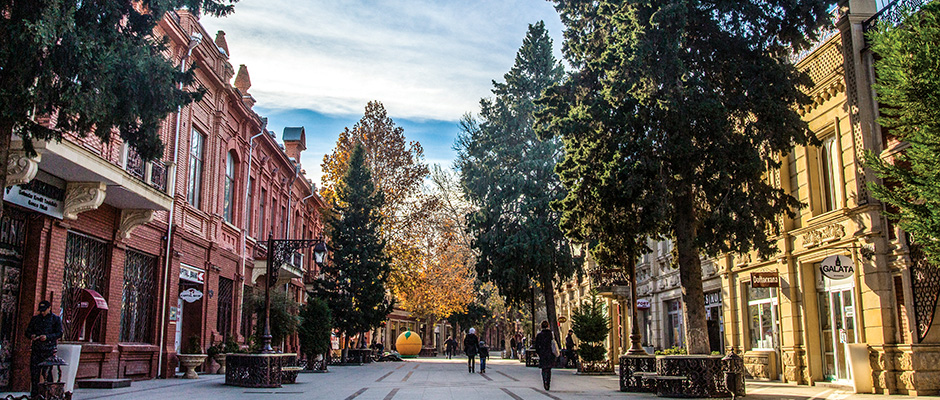
\includegraphics[width=11cm, height=6cm]{img/gence02.jpg}
        \caption{Javad Khan Street} 
    \end{figure}
  
\end{frame}

\begin{frame}{
\includegraphics[width=.9cm, height=1.2cm]{img/gence04.png}}
    \begin{figure}
        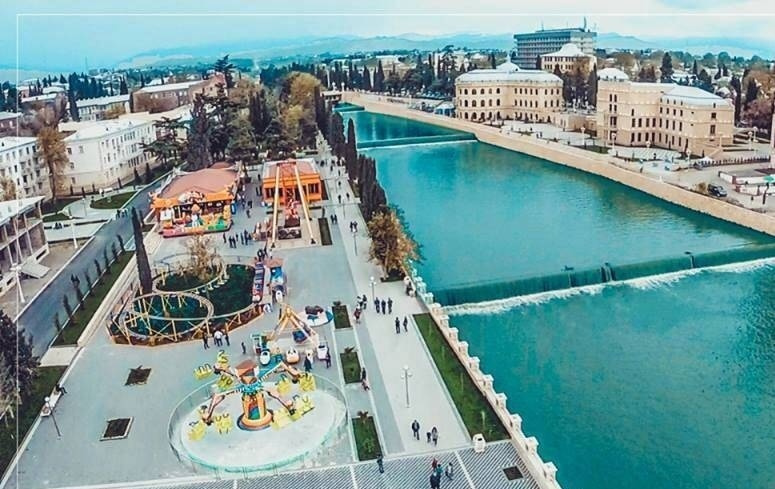
\includegraphics[width=11cm, height=6cm]{img/gence03.jpg}
        \caption{Ganja River} 
    \end{figure}
\end{frame}

\begin{frame}{Cities}
\begin{alertblock}{Sumqayit}
\justifying The third biggest city in Azerbaijan after Baku and Ganja. Population of Sumqayit is 341,200.
% Sumqayit has industries including metallurgical and chemical plants. \\
\end{alertblock}
\end{frame}

\begin{frame}{
\includegraphics[width=1.1cm, height=1.3cm]{img/sum04.png}}
    \begin{figure}
        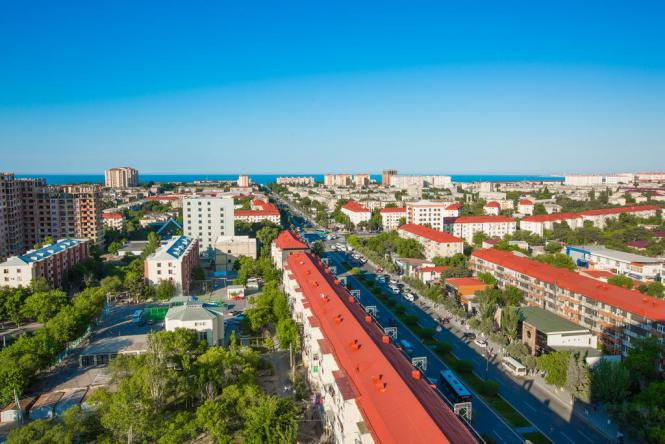
\includegraphics[width=11cm, height=6cm]{img/sum01.jpg}
        \caption{Sumqayit City View} 
    \end{figure}
\end{frame}

\begin{frame}{
\includegraphics[width=1.1cm, height=1.3cm]{img/sum04.png}}
    \begin{figure}
      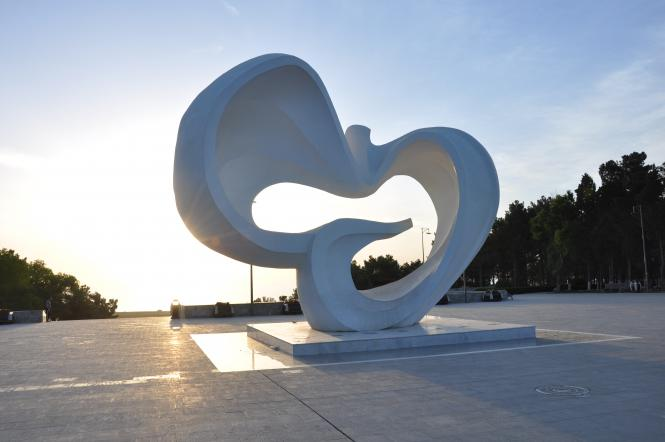
\includegraphics[width=11cm, height=6cm]{img/sum02.jpg}
        \caption{Sumqayit Peace Monument} 
    \end{figure}
\end{frame}

\begin{frame}{
\includegraphics[width=1.1cm, height=1.3cm]{img/sum04.png}}
    \begin{figure}
      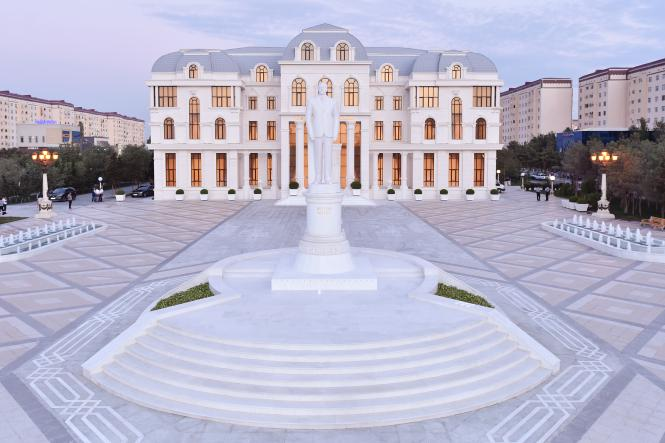
\includegraphics[width=11cm, height=6cm]{img/sum03.jpg}
        \caption{Center of Heydar Aliyev} 
    \end{figure}
\end{frame}

\begin{frame}{Landscape}
\begin{alertblock}{Landscape}
Azerbaijan is home to a vast variety of landscapes.
9 out of 11 existing climate zones are present in
Azerbaijan.
\end{alertblock}
\end{frame}


\begin{frame}{Landscape}
\begin{figure}
\begin{multicols}{2}
\centering
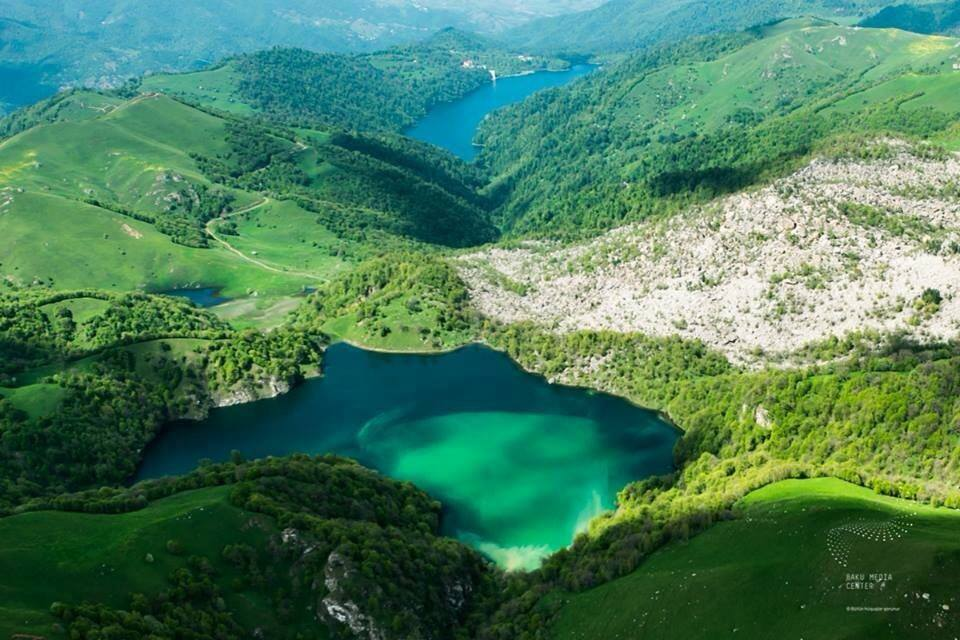
\includegraphics[width=4.5cm, height=2.4cm]{img/lake01.jpg}
 \caption{Qoygol Lake}

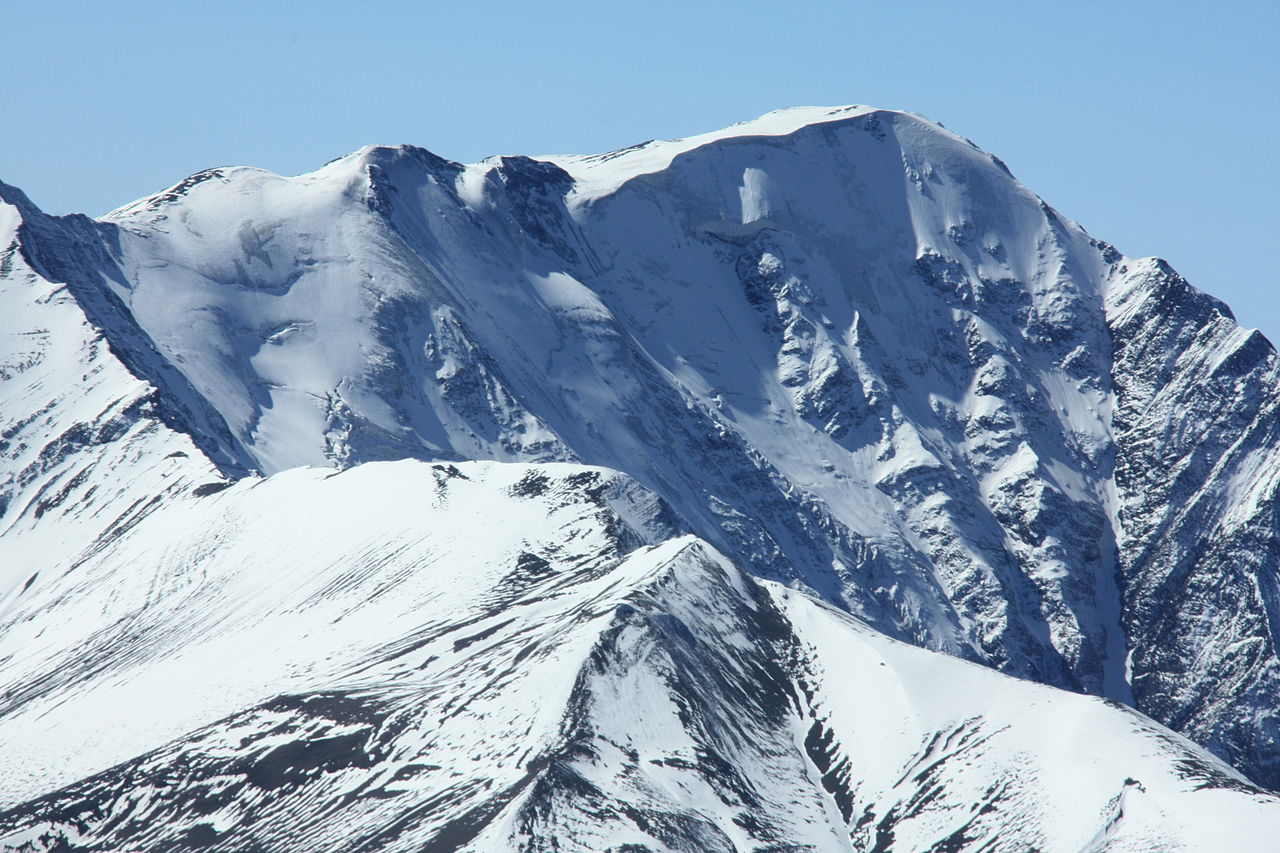
\includegraphics[width=4.5cm, height=2.4cm]{img/mount01.jpg}
 \caption{Murov Dag Mountain}
  \columnbreak
 
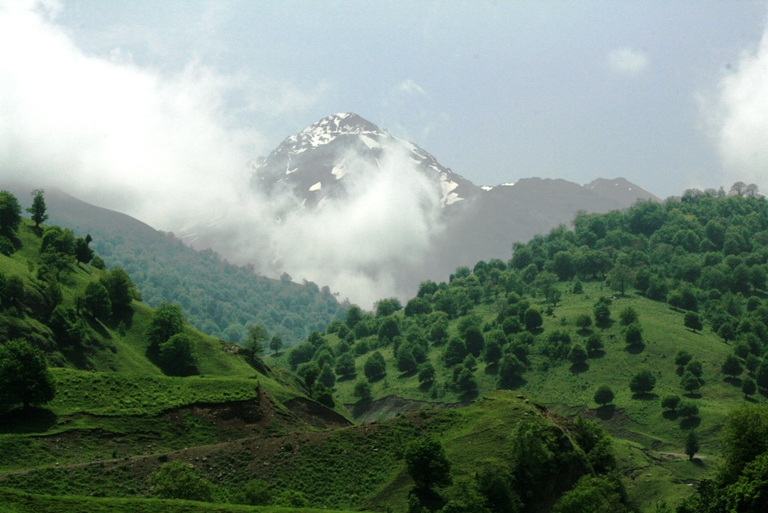
\includegraphics[width=4.5cm, height=2.4cm]{img/mount02.jpg}
\caption{Sakh Dag Mountain}

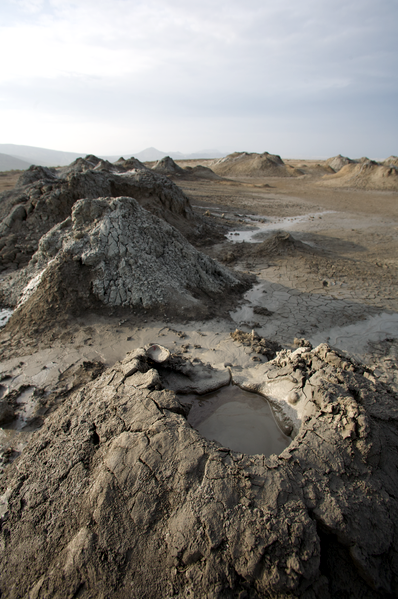
\includegraphics[width=4.5cm, height=2.4cm]{img/vul01.png}
\caption{Abseron Mud Volcano}
\end{multicols}
\end{figure}
\end{frame}

\begin{frame}{Cuisine}
\begin{alertblock}{Cuisine}
\justifying Azeri food features different dishes such as plov saffron-covered rice,kebabs. An array of seafood dishes, fresh-fruits, vegetables, and other dishes using herbs and spices.
\end{alertblock}
\end{frame}

\begin{frame}{Cuisine}
\begin{figure}
\begin{multicols}{2}
\centering
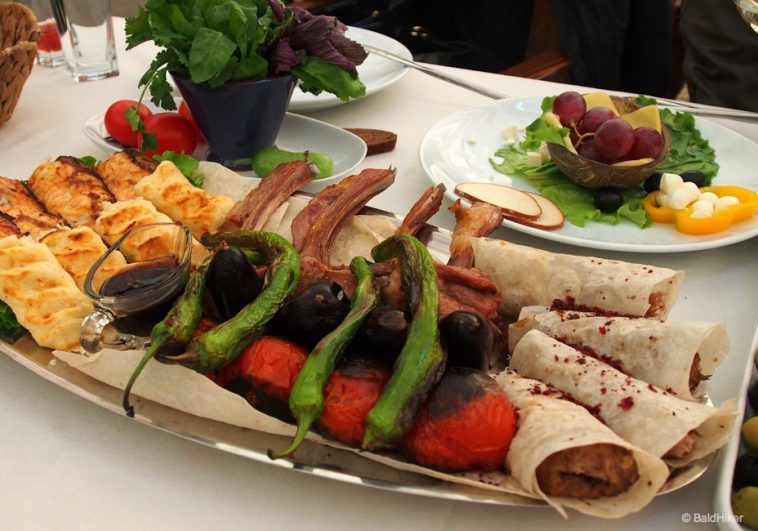
\includegraphics[width=4.5cm, height=2.4cm]{img/cus01.jpg}
 \caption{Kebab}

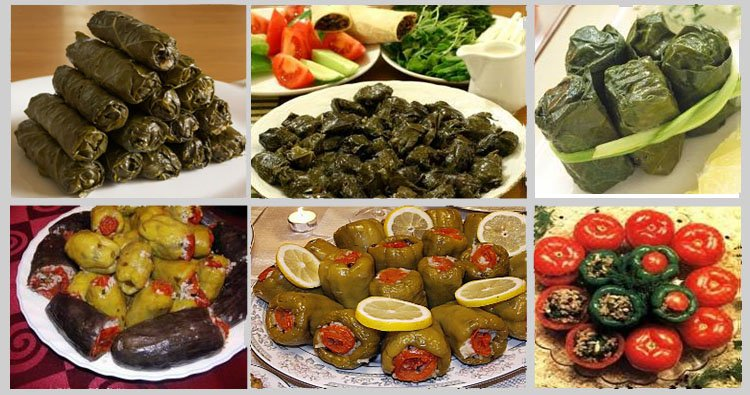
\includegraphics[width=4.5cm, height=2.4cm]{img/cus02.jpg}
 \caption{Dolma}
  \columnbreak
 
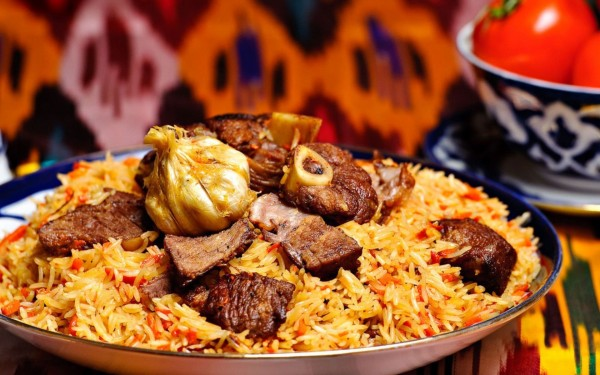
\includegraphics[width=4.5cm, height=2.4cm]{img/cus03.jpg}
\caption{Plov}

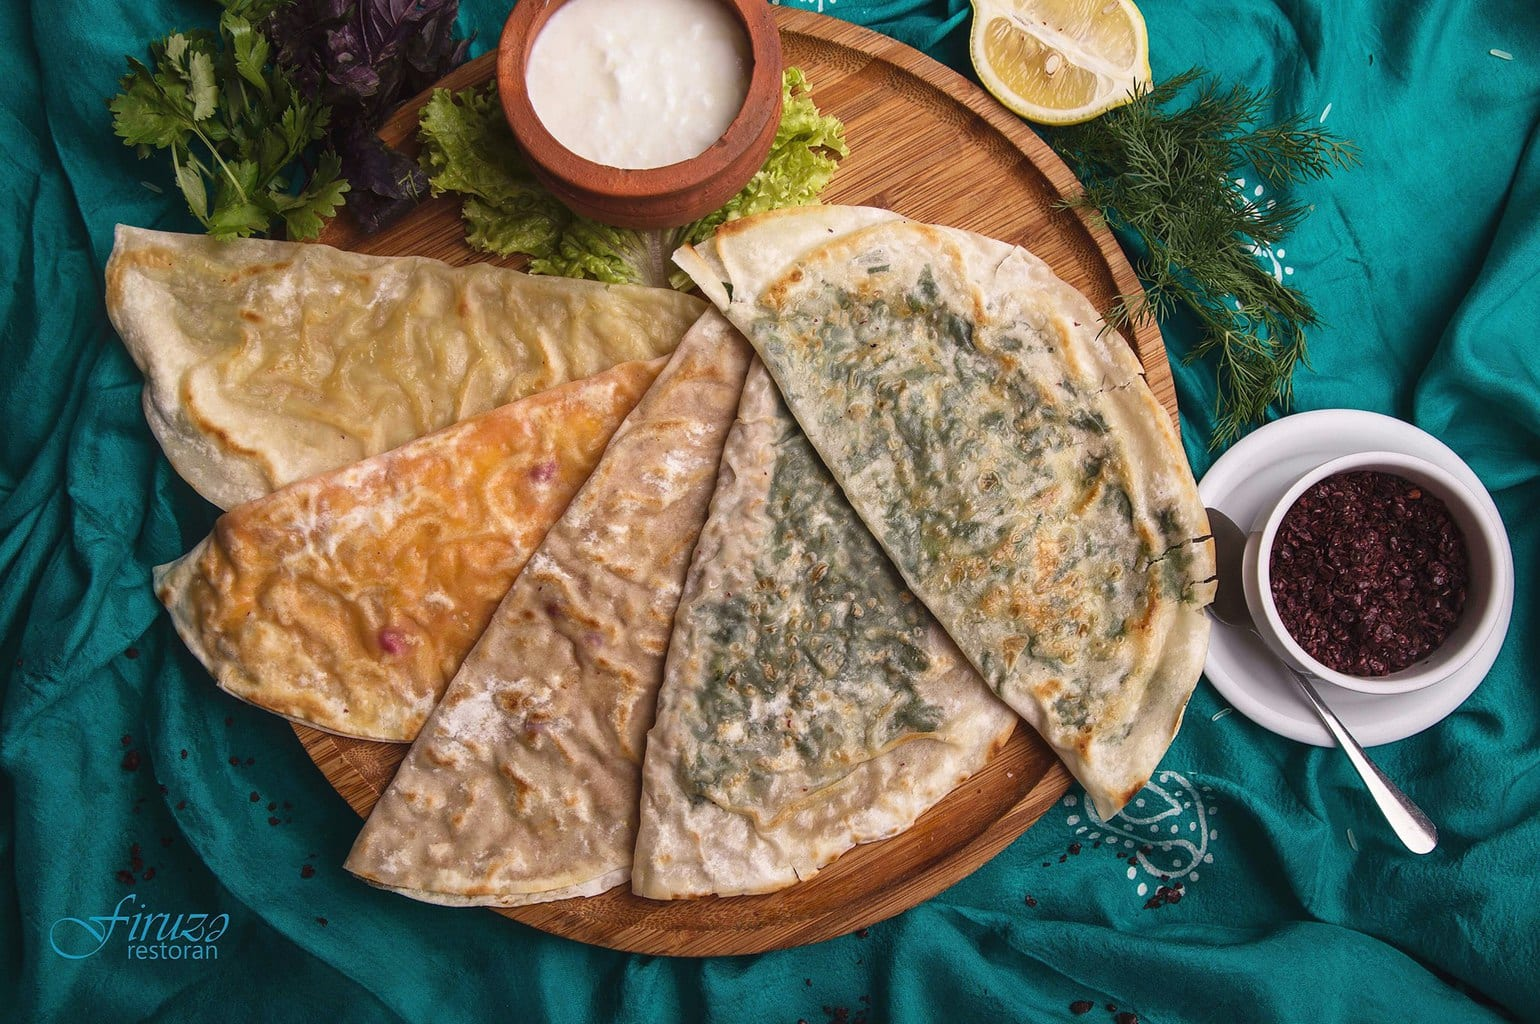
\includegraphics[width=4.5cm, height=2.4cm]{img/cus04.jpg}
\caption{Qutab}
\end{multicols}
\end{figure}
\end{frame}


\end{document}
